\section{Hiperfoco}

% ── Frame: Hiperfoco, ejemplo 1 (un solo objeto en primer plano) ─────────────
%  Las fotografías ya tienen bokeh óptico (poca profundidad de campo): no se
%  aplica ningún efecto adicional.
\begin{frame}{Hiperfoco: un solo objeto en primer plano}
  \begin{columns}[c,totalwidth=\textwidth]
    \begin{column}{0.58\textwidth}
      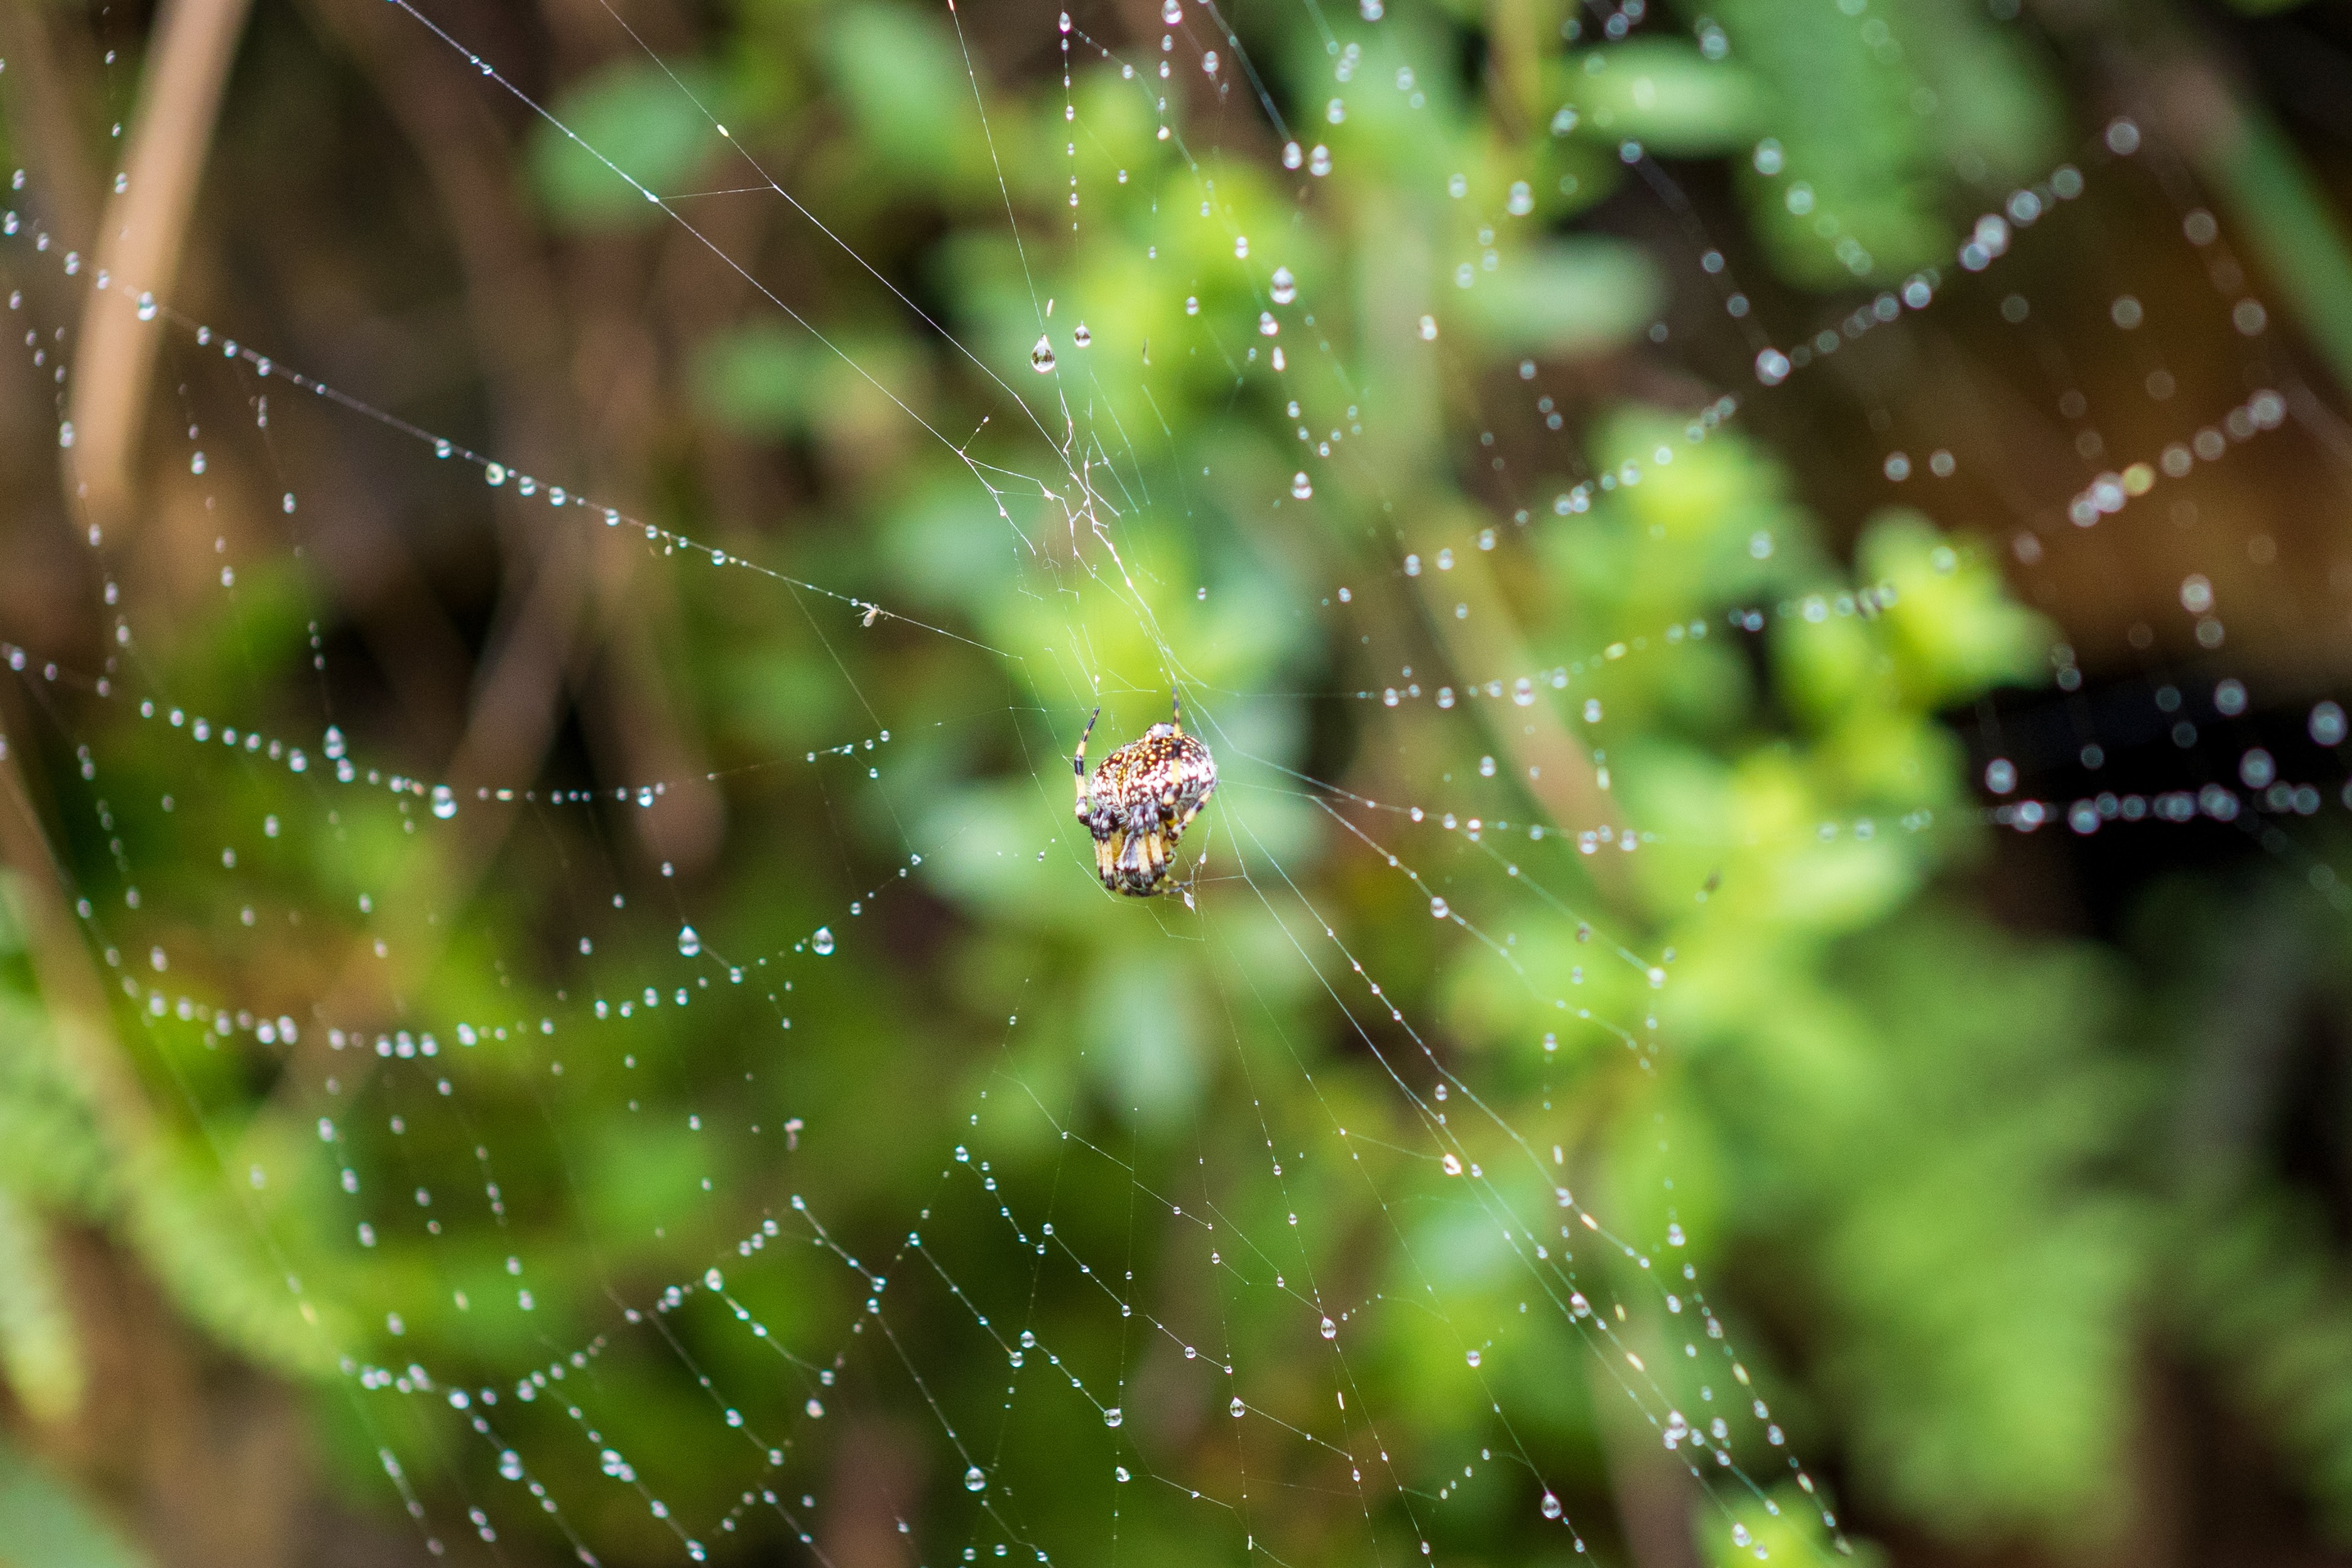
\includegraphics[width=\textwidth]{img/IMG_5321.jpeg}
      \fuentefigura{Fotografía de autoría propia; Bosques de Milpa Alta.}
    \end{column}
    \begin{column}{0.39\textwidth}
      \small
      {\itshape\color{ColorPrincipal}
        «una tendencia a concentrarse en profundidad con exclusión de otros
        estímulos»\par}
      {\raggedleft\footnotesize\color{gray!70} --- \citet[p.~34]{wood2021}\par}

      \vspace{0.3cm}
      {\itshape\color{ColorPrincipal}
        «durante un estado de hiperfoco hay una percepción disminuida de los
        estímulos no relevantes para la tarea»\par}
      {\raggedleft\footnotesize\color{gray!70} --- \citet{ashinoff2021}\par}

      \vspace{0.3cm}
      % EDITAR: explicación propuesta (redacción propia).
      La araña queda nítida; el resto de la escena sigue ahí, pero pierde
      definición.
    \end{column}
  \end{columns}
\end{frame}

% ── Frame: Hiperfoco, ejemplo 2 (el entorno se vuelve luces difusas) ─────────
\begin{frame}{Hiperfoco: el entorno se vuelve luces difusas}
  \begin{columns}[c,totalwidth=\textwidth]
    \begin{column}{0.58\textwidth}
      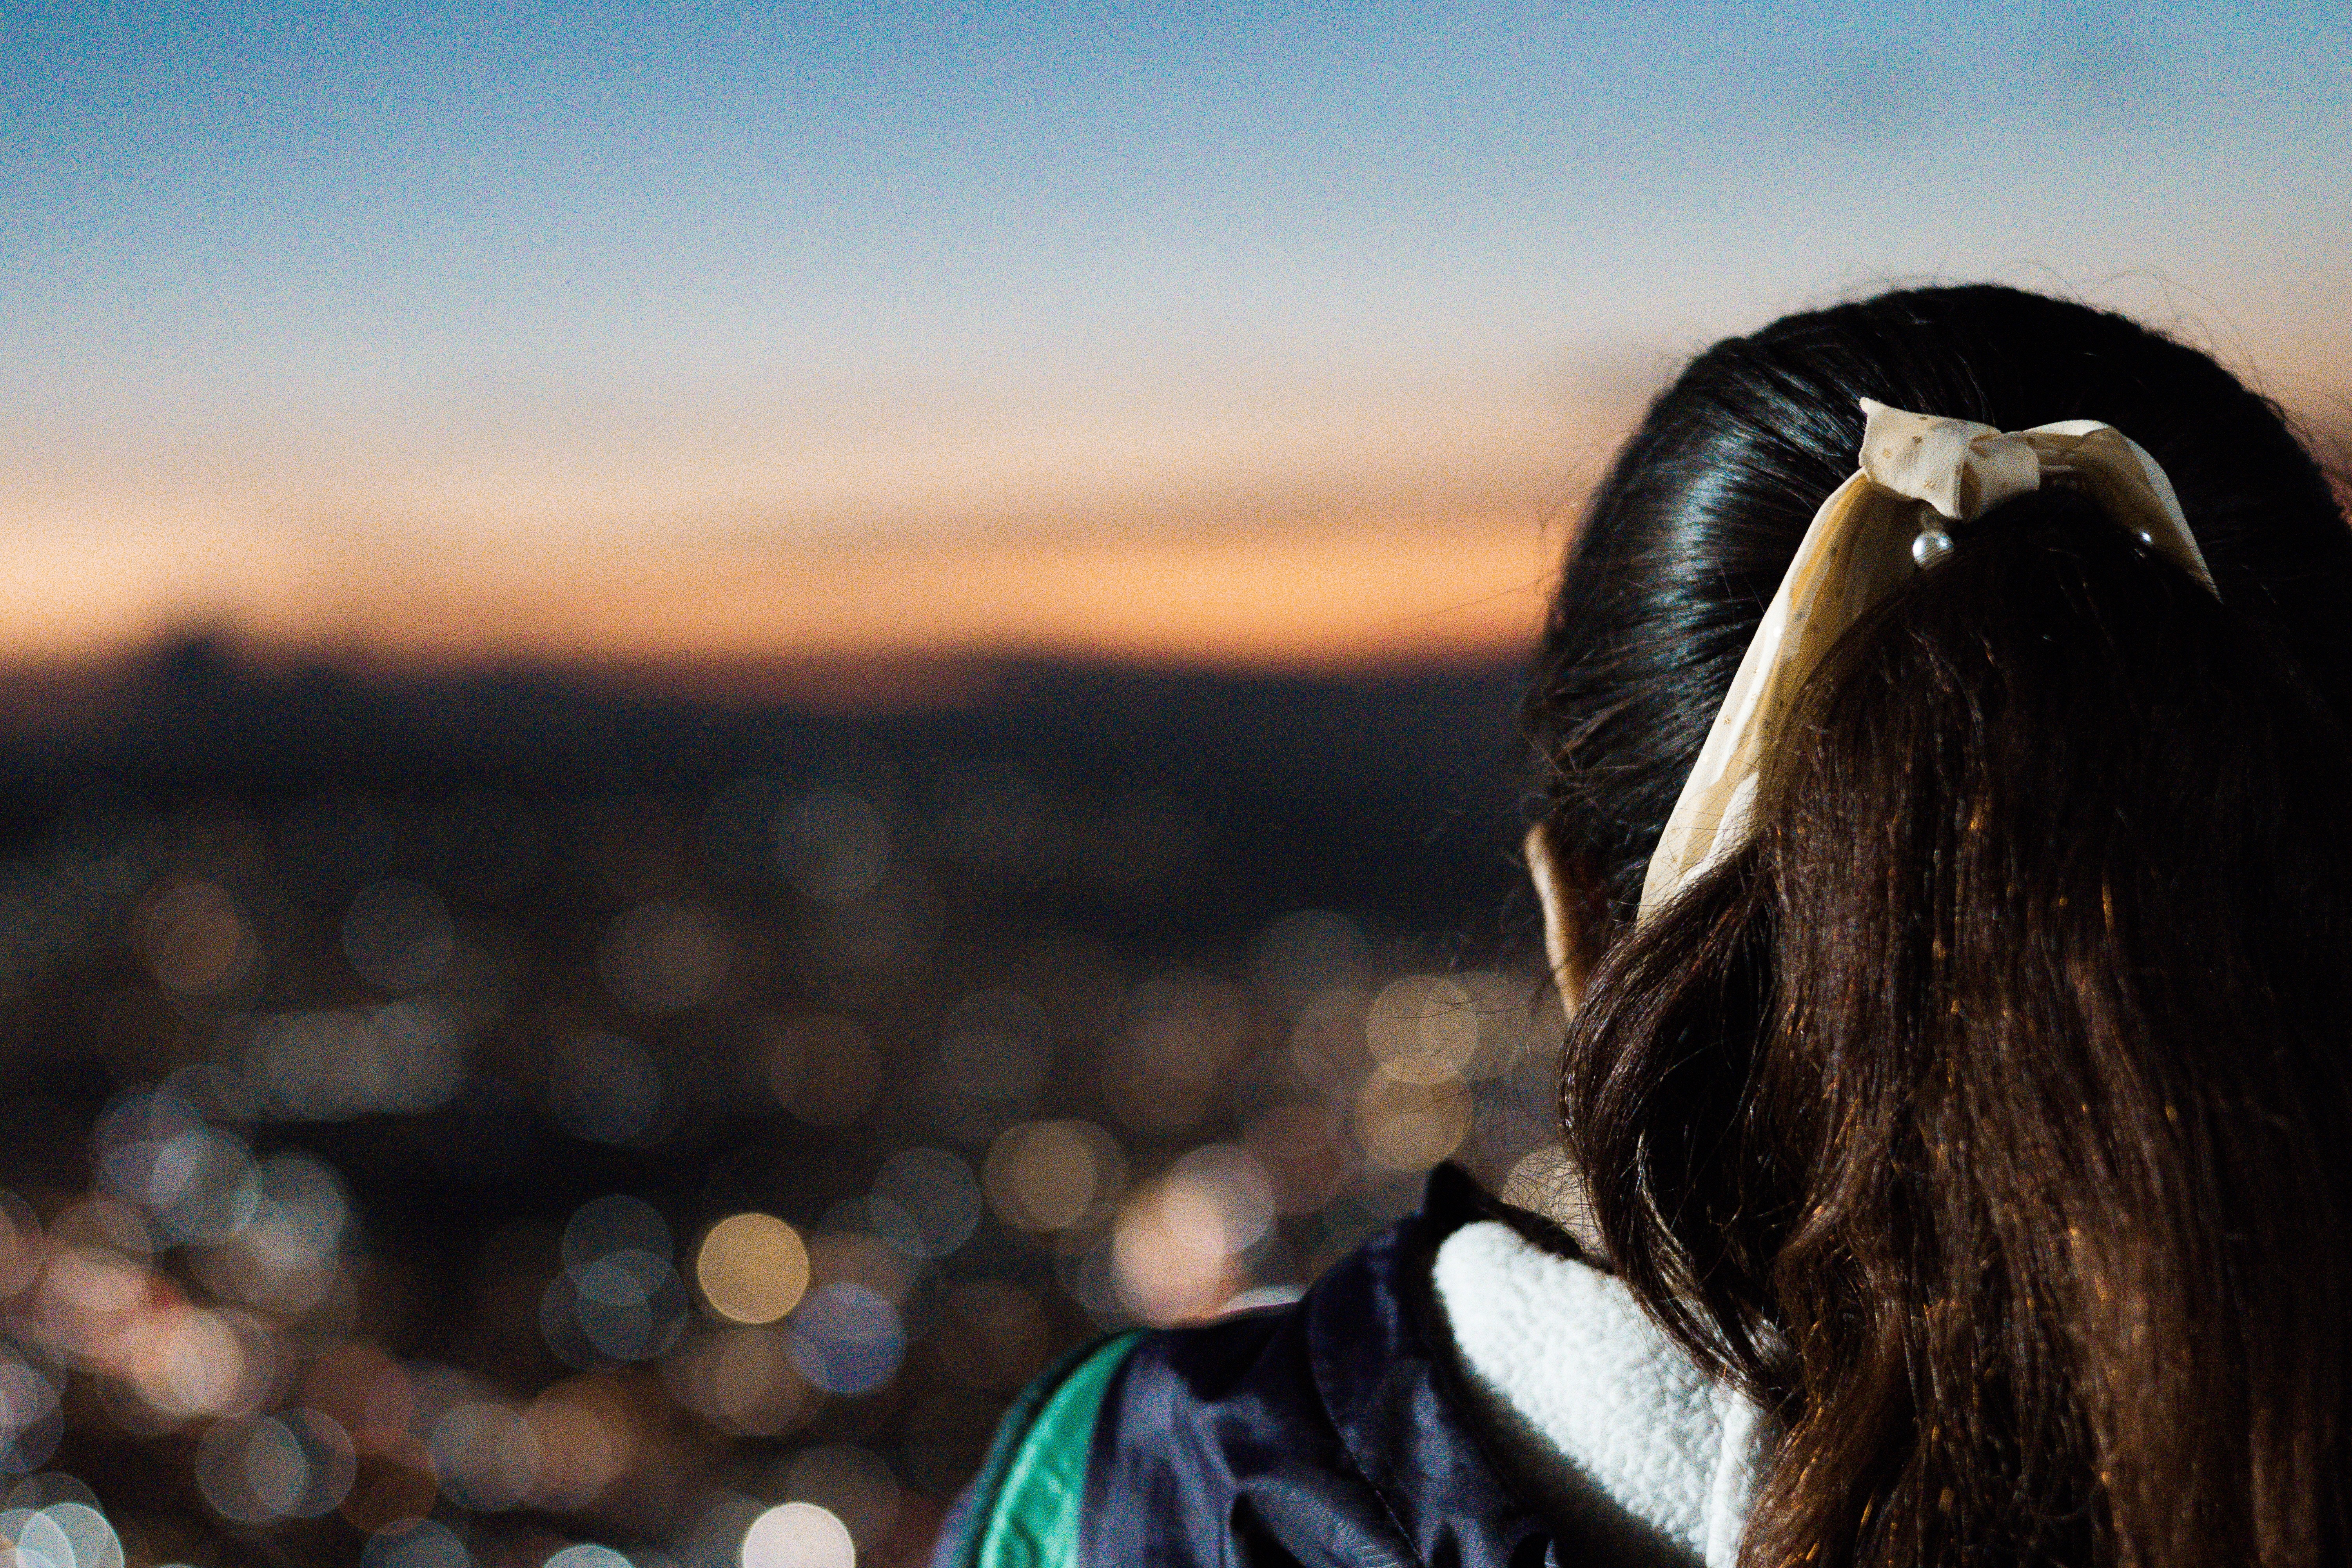
\includegraphics[width=\textwidth]{img/IMG_5357.jpeg}
      \fuentefigura{Fotografía de autoría propia; Catedral de Sal Zipaquirá en Colombia.}
      % EDITAR: autoría o fuente de la fotografía.
    \end{column}
    \begin{column}{0.39\textwidth}
      \small
      {\itshape\color{ColorPrincipal}
        «durante un estado de hiperfoco, el desempeño en la tarea mejora»\par}
      {\raggedleft\footnotesize\color{gray!70} --- \citet{ashinoff2021}\par}

      \vspace{0.3cm}
      {\itshape\color{ColorPrincipal}
        «la importancia de percibir esta disposición como una fortaleza, en
        lugar de un déficit que deba remediarse de algún modo»\par}
      {\raggedleft\footnotesize\color{gray!70} --- \citet{wood2021}\par}

      \vspace{0.3cm}
      % EDITAR: explicación propuesta (redacción propia).
      La ciudad no desaparece: se convierte en luces difusas mientras la
      atención se queda en un solo punto.
    \end{column}
  \end{columns}
\end{frame}


% ── Diapositivas a pantalla completa ─────────────────────────────────────────
%  Las imágenes se leen de la guía (Articulo1), sin duplicarlas.
%  \DiapositivaCompleta{ruta}{capa TikZ opcional}{nota del presentador}
%  Las notas (\note) no se proyectan; para verlas en una segunda pantalla:
%  \setbeameroption{show notes on second screen=right} en main.tex (pdfpc).
\providecommand{\RutaDinamicaTres}{../Articulo1/Resources/img/Dinamica3}
\providecommand{\DiapositivaCompleta}[3]{%
  {\setbeamertemplate{navigation symbols}{}% sin íconos de navegación
  \begin{frame}[plain]
    \begin{tikzpicture}[remember picture,overlay]
      \node at (current page.center)
        {\includegraphics[width=\paperwidth,height=\paperheight]{#1}};
      #2
    \end{tikzpicture}
    \note{#3}
  \end{frame}}}

% ── Frame: Antes de leer ─────────────────────────────────────────────────────
\begin{frame}{Antes de leer}
  \vfill
  \begin{center}
    {\Large\color{ColorPrincipal} Lean el texto e intenten retener los detalles.\par}
  \end{center}
  \vfill
  \note{Iniciar el audio (Audio\_Final\_Prueba.wav) desde 0:00 al pasar a la
  siguiente diapositiva.}
\end{frame}

% ── Fase 1: Odisea, Canto IX (audio 0:00 – 1:55, propuesta) ──────────────────
\DiapositivaCompleta{\RutaDinamicaTres/Fase1/Dinamica3_Fase1_Diapositiva1.png}{}
  {Audio 0:00 -- 1:55 (propuesta): base de oficina y pasillo. El grupo lee e
  intenta retener los detalles.}

\DiapositivaCompleta{\RutaDinamicaTres/Fase1/Dinamica3_Fase1_Diapositiva2.png}{}
  {Explicar que el hiperfoco permite ignorar la paja o el adorno social y
  literario para ir directo al núcleo de la información.}

% EDITAR: texto guía sobre el audio (redacción propia).
\DiapositivaCompleta{\RutaDinamicaTres/Fase1/Dinamica3_Fase1_Diapositiva3.png}
  {\node[anchor=south, text=white!75!black, font=\scriptsize]
     at ([yshift=0.3cm]current page.south)
     {El audio continúa. La siguiente lectura comenzará en unos minutos.};}
  {Se queda proyectada hasta 4:52, cuando comienza la Fase 2.}
